\documentclass[11pt]{article}
\usepackage{amssymb, amsthm, amsmath}
\usepackage{bm}
\usepackage{graphicx}
\usepackage[authoryear]{natbib}
\usepackage{bm}
\usepackage{verbatim}
\usepackage{lineno}
\usepackage{times}
\usepackage{soul}
\usepackage{color}

\usepackage[left=1in,top=1in,right=1in]{geometry}
\pdfpageheight 11in
\pdfpagewidth 8.5in
\linespread{1.0}
\newcommand{\btheta}{ \mbox{\boldmath $\theta$}}
\newcommand{\bmu}{ \mbox{\boldmath $\mu$}}
\newcommand{\balpha}{ \mbox{\boldmath $\alpha$}}
\newcommand{\bbeta}{ \mbox{\boldmath $\beta$}}
\newcommand{\bdelta}{ \mbox{\boldmath $\delta$}}
\newcommand{\blambda}{ \mbox{\boldmath $\lambda$}}
\newcommand{\bgamma}{ \mbox{\boldmath $\gamma$}}
\newcommand{\brho}{ \mbox{\boldmath $\rho$}}
\newcommand{\bpsi}{ \mbox{\boldmath $\psi$}}
\newcommand{\bepsilon}{ \mbox{\boldmath $\epsilon$}}
\newcommand{\bomega}{ \mbox{\boldmath $\omega$}}
\newcommand{\bOmega}{ \mbox{\boldmath $\Omega$}}
\newcommand{\bDelta}{ \mbox{\boldmath $\Delta$}}
\newcommand{\bSigma}{ \mbox{\boldmath $\Sigma$}}
\newcommand{\bPsi}{\mbox{\boldmath $\Psi$}}
\newcommand{\bOne}{\mbox{\boldmath $1$}}
\newcommand{\omu}{\overline{\mu}}
\newcommand{\oSigma}{\overline{\Sigma}}
\newcommand{\Yt}{{\tilde Y}}
\newcommand{\bA}{ \mbox{\bf A}}
\newcommand{\bP}{ \mbox{\bf P}}
\newcommand{\bx}{ \mbox{\bf x}}
\newcommand{\bX}{ \mbox{\bf X}}
\newcommand{\bB}{ \mbox{\bf B}}
\newcommand{\bZ}{ \mbox{\bf Z}}
\newcommand{\by}{ \mbox{\bf y}}
\newcommand{\bY}{ \mbox{\bf Y}}
\newcommand{\bz}{ \mbox{\bf z}}
\newcommand{\bh}{ \mbox{\bf h}}
\newcommand{\br}{ \mbox{\bf r}}
\newcommand{\bt}{ \mbox{\bf t}}
\newcommand{\bs}{ \mbox{\bf s}}
\newcommand{\bb}{ \mbox{\bf b}}
\newcommand{\bL}{ \mbox{\bf L}}
\newcommand{\bu}{ \mbox{\bf u}}
\newcommand{\bv}{ \mbox{\bf v}}
\newcommand{\bV}{ \mbox{\bf V}}
\newcommand{\bW}{ \mbox{\bf W}}
\newcommand{\bG}{ \mbox{\bf G}}
\newcommand{\bH}{ \mbox{\bf H}}
\newcommand{\bw}{ \mbox{\bf w}}
\newcommand{\bo}{ \mbox{\bf o}}
\newcommand{\bfe}{ \mbox{\bf e}}
\newcommand{\iid}{\stackrel{iid}{\sim}}
\newcommand{\indep}{\stackrel{indep}{\sim}}
\newcommand{\calR}{{\cal R}}
\newcommand{\calG}{{\cal G}}
\newcommand{\calD}{{\cal D}}
\newcommand{\calS}{{\cal S}}
\newcommand{\calB}{{\cal B}}
\newcommand{\calA}{{\cal A}}
\newcommand{\calT}{{\cal T}}
\newcommand{\calO}{{\cal O}}
\newcommand{\argmax}{{\mathop{\rm arg\, max}}}
\newcommand{\argmin}{{\mathop{\rm arg\, min}}}
\newcommand{\Frechet}{\mbox{Fr$\acute{\mbox{e}}$chet }}
\newcommand{\Matern}{\mbox{Mat$\acute{\mbox{e}}$rn }}
\newcommand{\ballunion}{B_a(\bs_1) \cup B_b(\bs_2) }

\newcommand{\beq}{ \begin{equation}}
\newcommand{\eeq}{ \end{equation}}
\newcommand{\beqn}{ \begin{eqnarray}}
\newcommand{\eeqn}{ \end{eqnarray}}


\begin{document}\linenumbers

\begin{center}
{\Large {\bf A new spatial model for points above a threshold}}\\
\today
\end{center}

\section{Introduction}\label{s:intro}
In most climatological applications, researchers are interested in learning about the average behavior of different climate variables (e.g. ozone, temperature, rainfall).
However, averages do not help regulators prepare for the unusual events that only happen once every 100 years.
For example, it is important to have an idea of how much rain will come in a 100-year floor in order to construct strong enough river levees to protect lands from flooding.

Unlike multivariate normal distributions, it is challenging to model multivariate extreme value distributions (e.g. generalized extreme value and generalized Pareto distribution) because few closed-form expressions exist for the density in more than two-dimensions \citep{Coles1991}.
Given this limitation, pairwise composite likelihoods have been used when modeling dependent extremes \citep{Padoan2010,Blanchet2011,Huser2013}.

One way around the multi-dimensional limitation of multivariate extreme value distributions is to use skew elliptical distributions to model dependent extreme values \citep{Genton2004,Zhang2010,Padoan2011}.
Due to their flexibility, the skew-normal and skew-$t$ distribution offer a flexible way to handle non-symmetric data within a framework of multivariate normal and multivariate t-distributions.
As with the spatial Gaussian process, the skew-normal distribution is also asymptotically independent; however, the skew-$t$ does demonstrate asymptotic dependence \citep{Padoan2011}.
Although asymptotic dependence is desirable between sites that are near one another, one drawback to the skew-$t$ is that sites remain asymptotically dependent even at far distances.

In this paper, we present a model that has marginal distributions with flexible tails, demonstrates asymptotic dependence for observations at sites that are near to one another, and has computation on the order of Gaussian models for large space-time datasets.
Specifically, our contribution is to incorporate thresholding and random spatial partitions using a multivariate skew-$t$ distribution.
The advantage of using a thresholded model as opposed to a non-thresholded model is that is allows for the tails of the distribution to inform the predictions in the tails \citep{DuMouchel1983}.
The random spatial partition alleviates the long-range spatial dependence seen by the skew-$t$.

The paper is organized as follows.
In section \ref{s:model}, we describe the skew-$t$ process with partitioning and thresholding.
The computing is described in section \ref{s:comp}.
In section \ref{s:simstudy}, we present a simulation study that examines the predictive capabilities of this model compared with a na\:{i}ve Gaussian method.
We then compare our method to Gaussian and max-stable methods with a data analysis of ozone measurements from the eastern US in section \ref{s:analysis}.
The final section provides brief discussion and direction for future research.

\section{Statistical model}\label{s:model}
Let $Y_t(\bs)\in \calR$ be the observed value at location $\bs$ and timepoint $t$.
To avoid bias in estimating tail parameters, we model censored data
\beq\label{Yt}
  \Yt_t(\bs) = \left\{
          \begin{array}{ll}
            Y_t(\bs) & Y_t(\bs)>T \\
            T & Y_t(\bs)\le T
          \end{array}
        \right.
\eeq
where $T$ is a pre-specified threshold.
Then, assuming the full data are observations from a skew-$t$ process, we update values censored below the threshold using standard Bayesian missing data methods as described in Section \ref{s:comp}.

\subsection{Skew-$t$ process}\label{s:data}
Many types of data demonstrate some level of skewness, and therefore should be modeled with distributions that allow for non-symmetry.
The skew-elliptical family of distributions provides models that are mathematically tractable while introducing additional paremeters to account for non-symmetric data \citep{Genton2004}.
One member of this family, is the skew-$t$ distribution \citep{Azzalini2003}.
We assume the data can be modeled using a skew-$t$ distribution.
\citet{Zhang2010} show that the skew-$t$ can be expressed as a hierarchical model
\begin{align} \label{eq:fullmodel}
  Y_t(\bs) &= X_t(\bs) \beta + \alpha |z_t| + \sigma_t v_t(\bs)
\end{align}
where $\alpha \in \calR$ controls the skewness, $z_{t} \ind N(0, \sigma^2_t)$ are a random effect from a half-normal distribution (see appendix A.4), $v_t(\bs)$ is a Gaussian process with mean zero, variance one, \Matern correlation, and $\sigma^2_t \iid \text{IG}(a, b)$.
When marginalizing over the $z_t$ and $\sigma^2_t$ terms,
\begin{align*}
  Y_t(\bs) \sim \text{skew-}t (\mu, \Sigma^*, \alpha, \text{df} = 2a)
\end{align*}
where $\mu$ is the location, $\Sigma^* = \frac{ b }{ a } \Sigma$, $\Sigma$ is a \Matern covariance matrix, and $\alpha \in \calR$ controls the skewness.
The skew-$t$ process is desirable because of its flexible tail that is controlled by the skewness parameter, $\alpha$, and the degrees of freedom, $2a$.
Furthermore, if $\bY$ follows a multivariate skew-$t$ distribution, the marginal distributions also follow a skew-$t$ distribution \citep{Azzalini2003}.

\subsection{Extremal dependence}
One common measure of extremal spatial dependence is the extremal coefficient which describes the pairwise dependence between spatial locations \citep{Smith1990}.
Consider a spatial process $Y(\bs) \in \calR^n$ observed at locations $s \in \calD \subset \calR^2$.
Then the bivariate extremal coefficient, $\theta(\bs_i, \bs_j) \in [1, 2]$, is defined as
\begin{align}
  \Pr(Y(\bs_i) < c, Y(\bs_j) < c) = \Pr(Y(\bs_i) < c)^{\theta(\bs_i, \bs_j) }. \label{eq:extremalcoef}
\end{align}
One way to characterize the dependence over the entire set of spatial locations is to calculate all of the pairwise extremal coefficients.
Although this method provides information regarding the spatial structure of the observations, it does not fully characterize the joint spatial dependence.

Another measure of extremal dependence is the $\chi$ statistic.
The $\chi$ statistic for the upper tail is given by
\begin{align*}
  \chi = \lim_{c \rightarrow \infty} \Pr(Y(\bs_1) > c | Y(\bs_2) > c),
\end{align*}
In a stationary spatial process, we can write the $\chi$ coefficient as
\begin{align*}
  \chi(\bh) = \lim_{c \rightarrow \infty} \Pr(Y(0) > c | Y(\bh) > c)
\end{align*}
where $\bh = ||\bs_1 - \bs_2||$.
If $\chi(\bh) = 0$, then observations are asymptotically independent at distance $\bh$.
For Gaussian processes, $\chi(\bh) = 0$ regardless of the the distance, so they are not suitable for modeling spatially dependent extremes.
However, for the process described in Section \ref{s:data}, $\chi(\bh) > 0$ \citep{Padoan2011}.

\subsection{Random daily partition}\label{s:part}
One problem with the spatial skew-$t$ process is that all sites are asymptotically dependent regardless of their spatial separation.
This occurs because all observations, both near and far, share the same $z_t$ and $\sigma^2_t$ terms.
We handle this problem with a daily random partition similar to \citet{Kim2005} that allows $z_t$ and $\sigma^2_t$ to vary by site.
The model then becomes
\begin{align}
  Y_t(\bs) &= X_t(\bs) \beta + \alpha |z_t(\bs)| + \sigma_t(\bs) v_t(\bs).
\end{align}
In this extension of (\ref{eq:fullmodel}), $z_t(\bs)$ and $\sigma_t(\bs)$ are allowed to vary by site.
Their spatial variation is determined by the random partition model defined below.
Consider a set of daily spatial knots $\bw_{tk} \sim \text{Uniform}(\calD)$ that define a random daily partition $P_{t1}, \ldots, P_{tK}$ of the spatial domain of interest $\calD \subset \calR^2$ such that
\begin{align*}
  P_{tk} = \{ \bs : k = \argmin_\ell || \bs - \bw_{t\ell} || \}.
\end{align*}
So, for $\bs \in P_{tk}$, let
\begin{align}
  z_t(\bs) &= z_{tk} \label{eq:sitez}\\
  \sigma^2_t(\bs) &= \sigma^2_{tk} \label{eq:sitesig}.
\end{align}
Then within each partition, $Y_t(\bs)$ follows the distribution given in (\ref{eq:fullmodel}).
When incorporating the random daily partition, the $\chi$ statistic becomes
\begin{align}
  \chi(\bh) = \lim_{c \rightarrow \infty} \pi(\bh) \chi(\bh)
\end{align}
where $\pi(h)$ is the probability that two sites separated by distance $h$ are in the same partition.
Asymptotic dependence is eliminated as $h$ increases, because
\begin{align}
  \lim_{h \rightarrow \infty} \chi(\bh) = \lim_{h \rightarrow \infty} \pi(\bh) \chi(\bh) = 0.
\end{align}
A proof of this can be found in Appendix A.3.

\subsection{Accounting for temporal dependence} \label{s:temporal}
In a standard block-maxima approach, the temporal dependence is assumed to be negligible because blocks (e.g. yearly maxima) are taken to be large enough to assume independence.
However, when using daily meausrements, the assumption of temporal independence is no longer appropriate.
We account for temporal dependence through an AR(1) time series on the spatial knots, $z_t(\bs)$ terms, and $\sigma^2_t(\bs)$ terms.
We first, transform the spatial knots from $\calD$ to $\calR^2$ as follows.
Let
\begin{align*}
  \bw^*_k = \Phi^{-1}_2\left[ \frac{ (\bw_k - \min(\bs))}{ \text{range}(\bs) } \right].
\end{align*}
where $\Phi_2$ represents a bivariate standard normal density function.
Then $\bw^*_k \in \calR^2$.
We use a copula on the $\sigma^2_t(\bs)$ to ensure that the marginal distributions of $\sigma^2_t(\bs)$ are inverse gamma.
Let
\begin{align*}
  \sigma^{2*}_t(\bs) =\Phi^{-1}\left\{ \text{IG}[\sigma^2_t(\bs)] \right\}
\end{align*}
where $\Phi$ is a univariate standard normal density function, and IG is the distribution function for an IG$(a, b)$ random variable.
Then the time series is modeled as
\begin{align}
  \bw^*_{t, k} | \bw^*_{t-1, k} &\sim N_2\left[\phi_w \bw^*_{t-1, k}, (1 - \phi_w^2) \right] \\
  z_{t, k} | z_{t-1, k} &\sim N \left[\phi_z z_{t-1, k}, \sigma^2_{t,k} (1 - \phi_z^2)\right] \\
  \sigma^{2*}_{t, k} | \sigma^{2*}_{t-1, k} &\sim N \left[\phi_\sigma \sigma^{2*}_{t-1, k}, (1 - \phi_\sigma^2) \right]
\end{align}
where $|\phi_w| < 1$, $0 < \phi_z < 1$, and $|\phi_\sigma| < 1$.

\subsection{Hierarchical model}\label{s:hier}
Conditioned on $z_{t,k}(\bs) \iid $ $N(0, \sigma^2_{t,k})$, $\sigma^2_{t,k}(\bs) \sim IG(a, b)$, and $P_{t,k}$, the marginal distributions are skew-$t$ and the joint distribution within a partition is multivariate skew-$t$.
However, we do not fix the partitions, they are treated as unknown and updated in the MCMC.
We model this with a Bayesian hierarchical model as follows.
Let $\bw_{t,1}, \ldots, \bw_{t,K}$ be a set of daily spatial knots in a spatial domain of interest, $\calD$, so that
\begin{align*}
 P_{t,k} = \{\bs : k = \argmin_\ell || \bs_t - \bw_{t\ell} ||\}.
\end{align*}

Then
\begin{align}
   Y_t(\bs) \mid z_{t}(\bs), \sigma^2(\bs), P_{t,k}, \alpha, \beta, \Theta &= X_t(\bs) \beta + \alpha |z_t(\bs)| + \sigma_t(\bs) v_t(\bs) \label{eq:hier}\\
   z_t(\bs) &= z_{t,k} \text{ if } \bs \in P_{t,k}\\
   \sigma^2_{t}(\bs) &= \sigma^2_{t,k} \text{ if } \bs \in P_{t,k}\\
   \alpha &\sim N(0, 10)\\
   v_t(\bs) \mid \Theta &\sim \Matern(0, \Sigma)\\
   z_{t,k} \mid z_{t-1, k}, \sigma^2_{tk} &\sim N(\phi_z z_{t-1, k}, \sigma^2_{t,k} (1 - \phi_z^2))\\
   \sigma^{2*}_{t,k} \mid \sigma^{2*}_{t-1, k} &\sim N(\phi_\sigma \sigma^{2*}_{t-1, k}, (1 - \phi_\sigma^2))\\
   \bw^*_{t,k} \mid \bw^*_{t-1, k} &\sim N_2(\phi_w \bw^*_{t-1, k}, (1 - \phi_w^2))
\end{align}
where $\Theta = \{\rho, \nu, \gamma\}$; \mbox{$k = \argmin_\ell ||\bs - \bw_\ell ||$}; and $\Sigma$ is a \Matern covariance matrix with variance one, spatial range $\rho$, smoothness $\nu$, and the proportion of variance accounted for by the spatial variation is $\gamma$.

\section{Computation}\label{s:comp}
The MCMC for this model is fairly straightforward.
First, we impute values below the threshold.
Then, we update $\Theta$ using random walk MH or Gibbs sampling when appropriate.
Finally, we make spatial predictions using conditional multivariate normal results and the fact that the distribution of $Y_t(\bs) \mid \Theta, z_{tl}$ is the usual multivariate normal distribution with a \Matern spatial covariance structure.

We can use Gibbs sampling to update $Y_t(\bs)$ for censored observations that are below the threshold $T$.
After conditioning on $\alpha$, $z_t(\bs)$ and non-censored observations, $Y_t(\bs)$ has truncated normal full conditionals.
So we sample $Y_t(\bs) \sim N_{(-\infty, T)}(\mu(\bs), \Sigma)$.
After imputing the censored observations, we update the model parameters.
To update the model parameters, we use standard Gibbs updates for parameters when possible.
In the case Gibbs sampling is not possible, parameters are updated using a random-walk Metropolis Hastings algorithm.
See Appendices A.1 and A.2 for details regarding the MCMC.
The final step of the computation is to use Bayesian Kriging to generate a predictive distribution for $Y_t(\bs^*)$ at prediction location $(\bs^*)$.
This step is similar to the imputation for censored observations except that the full conditionals are no longer truncated at $T$.

\section{Simulation study}\label{s:simstudy}
In this section, we conduct a simulation study to investigate how the number of partitions and the level of thresholding impact the accuracy of predictions made by the model.

\subsection{Design}\label{s:simdesign}
For all simulation designs, we generate data from the model presented in Section \ref{s:part} using $n_s=130$ sites and $n_t=50$ independent days.
The sites are generated Uniform$([0, 10] \times [0, 10])$.
We generate data from 6 different simulation designs:
\begin{enumerate} \setlength{\itemsep}{-0.5em}
  \item Gaussian marginal, $K=1$ knot
  \item $t$ marginal, $K=1$ knot
  \item $t$ marginal, $K=5$ knots
  \item skew-$t$ marginal, $K=1$ knots
  \item skew-$t$ marginal, $K=5$ knots
  \item Max-stable.
\end{enumerate}
In the first five designs, the $v_t(\bs)$ terms are generated using a \Matern covariance with smoothness parameter, $\nu = 0.5$, and spatial range, $\rho = 0.1$.
For the covariance matrices in designs 1 -- 5, the proportion of the variance accounted for by the spatial variation is $\gamma = 0.9$ while the proportion of the variance accounted for by the nugget effect is $0.1$.
In the first design, $\sigma^2 = 2$ is used for all days.
For designs 2 -- 4, $\sigma^2_{tk} \iid \text{IG}(3, 8)$
For designs 1 -- 3, we set $\alpha = 0$.
For designs four and five, $\alpha = 3$ was used, and the $z_t$ are generated as described in (\ref{eq:sitez}).
In the sixth design, we generate from a spatial max-stable distribution \citep{Reich2012} with parameters $\mu = 1, \sigma=1, \xi=0.2$ and 144 spatial knots on a regular lattice in the square $[1, 9] \times [1, 9]$.
In all six designs, the mean ($\mu(\bs)$) is assumed to be constant across space.

$M = 50$ data sets are generated for each design.
For each data set we fit the data using
\begin{enumerate} \setlength{\itemsep}{-0.5em}
  \item Gaussian marginal, $K=1$ knots
  \item skew-$t$ marginal, $K=1$ knots, $T=-\infty$
  \item $t$ marginal, $K=1$ knots, $T=q(0.80)$
  \item skew-$t$ marginal, $K=5$ knots, $T=-\infty$
  \item $t$ marginal, $K=5$ knots, $T=q(0.80)$
\end{enumerate}
where $q(0.80)$ is the 80th sample quantile of the data.
The design matrix $\bX$ includes an the intercept with a prior of $\beta \sim \text{N}(0, 10)$.
The spatial covariance parameters have priors $\log(\nu) \sim \text{N}(-1.2, 1)$, $\gamma \sim \text{U}(0, 1)$, $\log(\rho) \sim \text{N}(-2, 1)$.
The skewness parameter has prior $\alpha \sim \text{N}(0, 2)$.
The residual variance terms have priors $\sigma^2_t(\bs) \sim \text{IG}(0.1, 0.1)$.

\subsection{Cross validation}\label{s:modelselect}
Models were compared using cross validation with 100 sites used as training sites and 30 sites witheld for testing.
The model was fit using the training set, and predictions were generated at the testing site locations.
Because one of the primary goals of this model is to predict extreme events, we quantify use Brier scores and quantile scores to select the model that best fits the data \citep{Gneiting2007}.
The Brier score for predicting exceedance of a threshold $c$ is given by $[e(c) - P(c)]^2$ where $e(c) = I[y>c]$ is an indicator function indicating that a test set value, $y$, has exceeded the threshold, $c$, and $P(c)$ is the predicted probability of exceeding $c$.
The quantile score for the $\tau$th quantile is $2\{ I[y < \widehat{q}(\tau)] - \tau\} (\widehat{q}(\tau) - y)$ where $y$ is a test set value and $\widehat{q}(\tau)$ is the estimated $\tau$th quantile.
For both the Brier score and the quantile score, a lower score indicates a better fit.
These scores were averaged over all sites and days to obtain a single quantile score for each dataset.

\subsection{Results}\label{s:simresults}
When comparing quantile scores, in almost all of the data settings, the biggest gains are seen when using thresholded methods.
In all data settings except for the max-stable setting, method 3 performs the best.
However, in most of the data settings, method 5 also performs reasonably well.
In fact, for setting 5, paired $t$-tests suggest that the difference in performance is not significant for any quantile score.
Furthermore, paired $t$-tests results indicate that the difference in quantile scores between methods 3 and 5 is only statistically significant after q(0.97) for setting 4 and after q(0.93) for setting 1.

\begin{figure}
  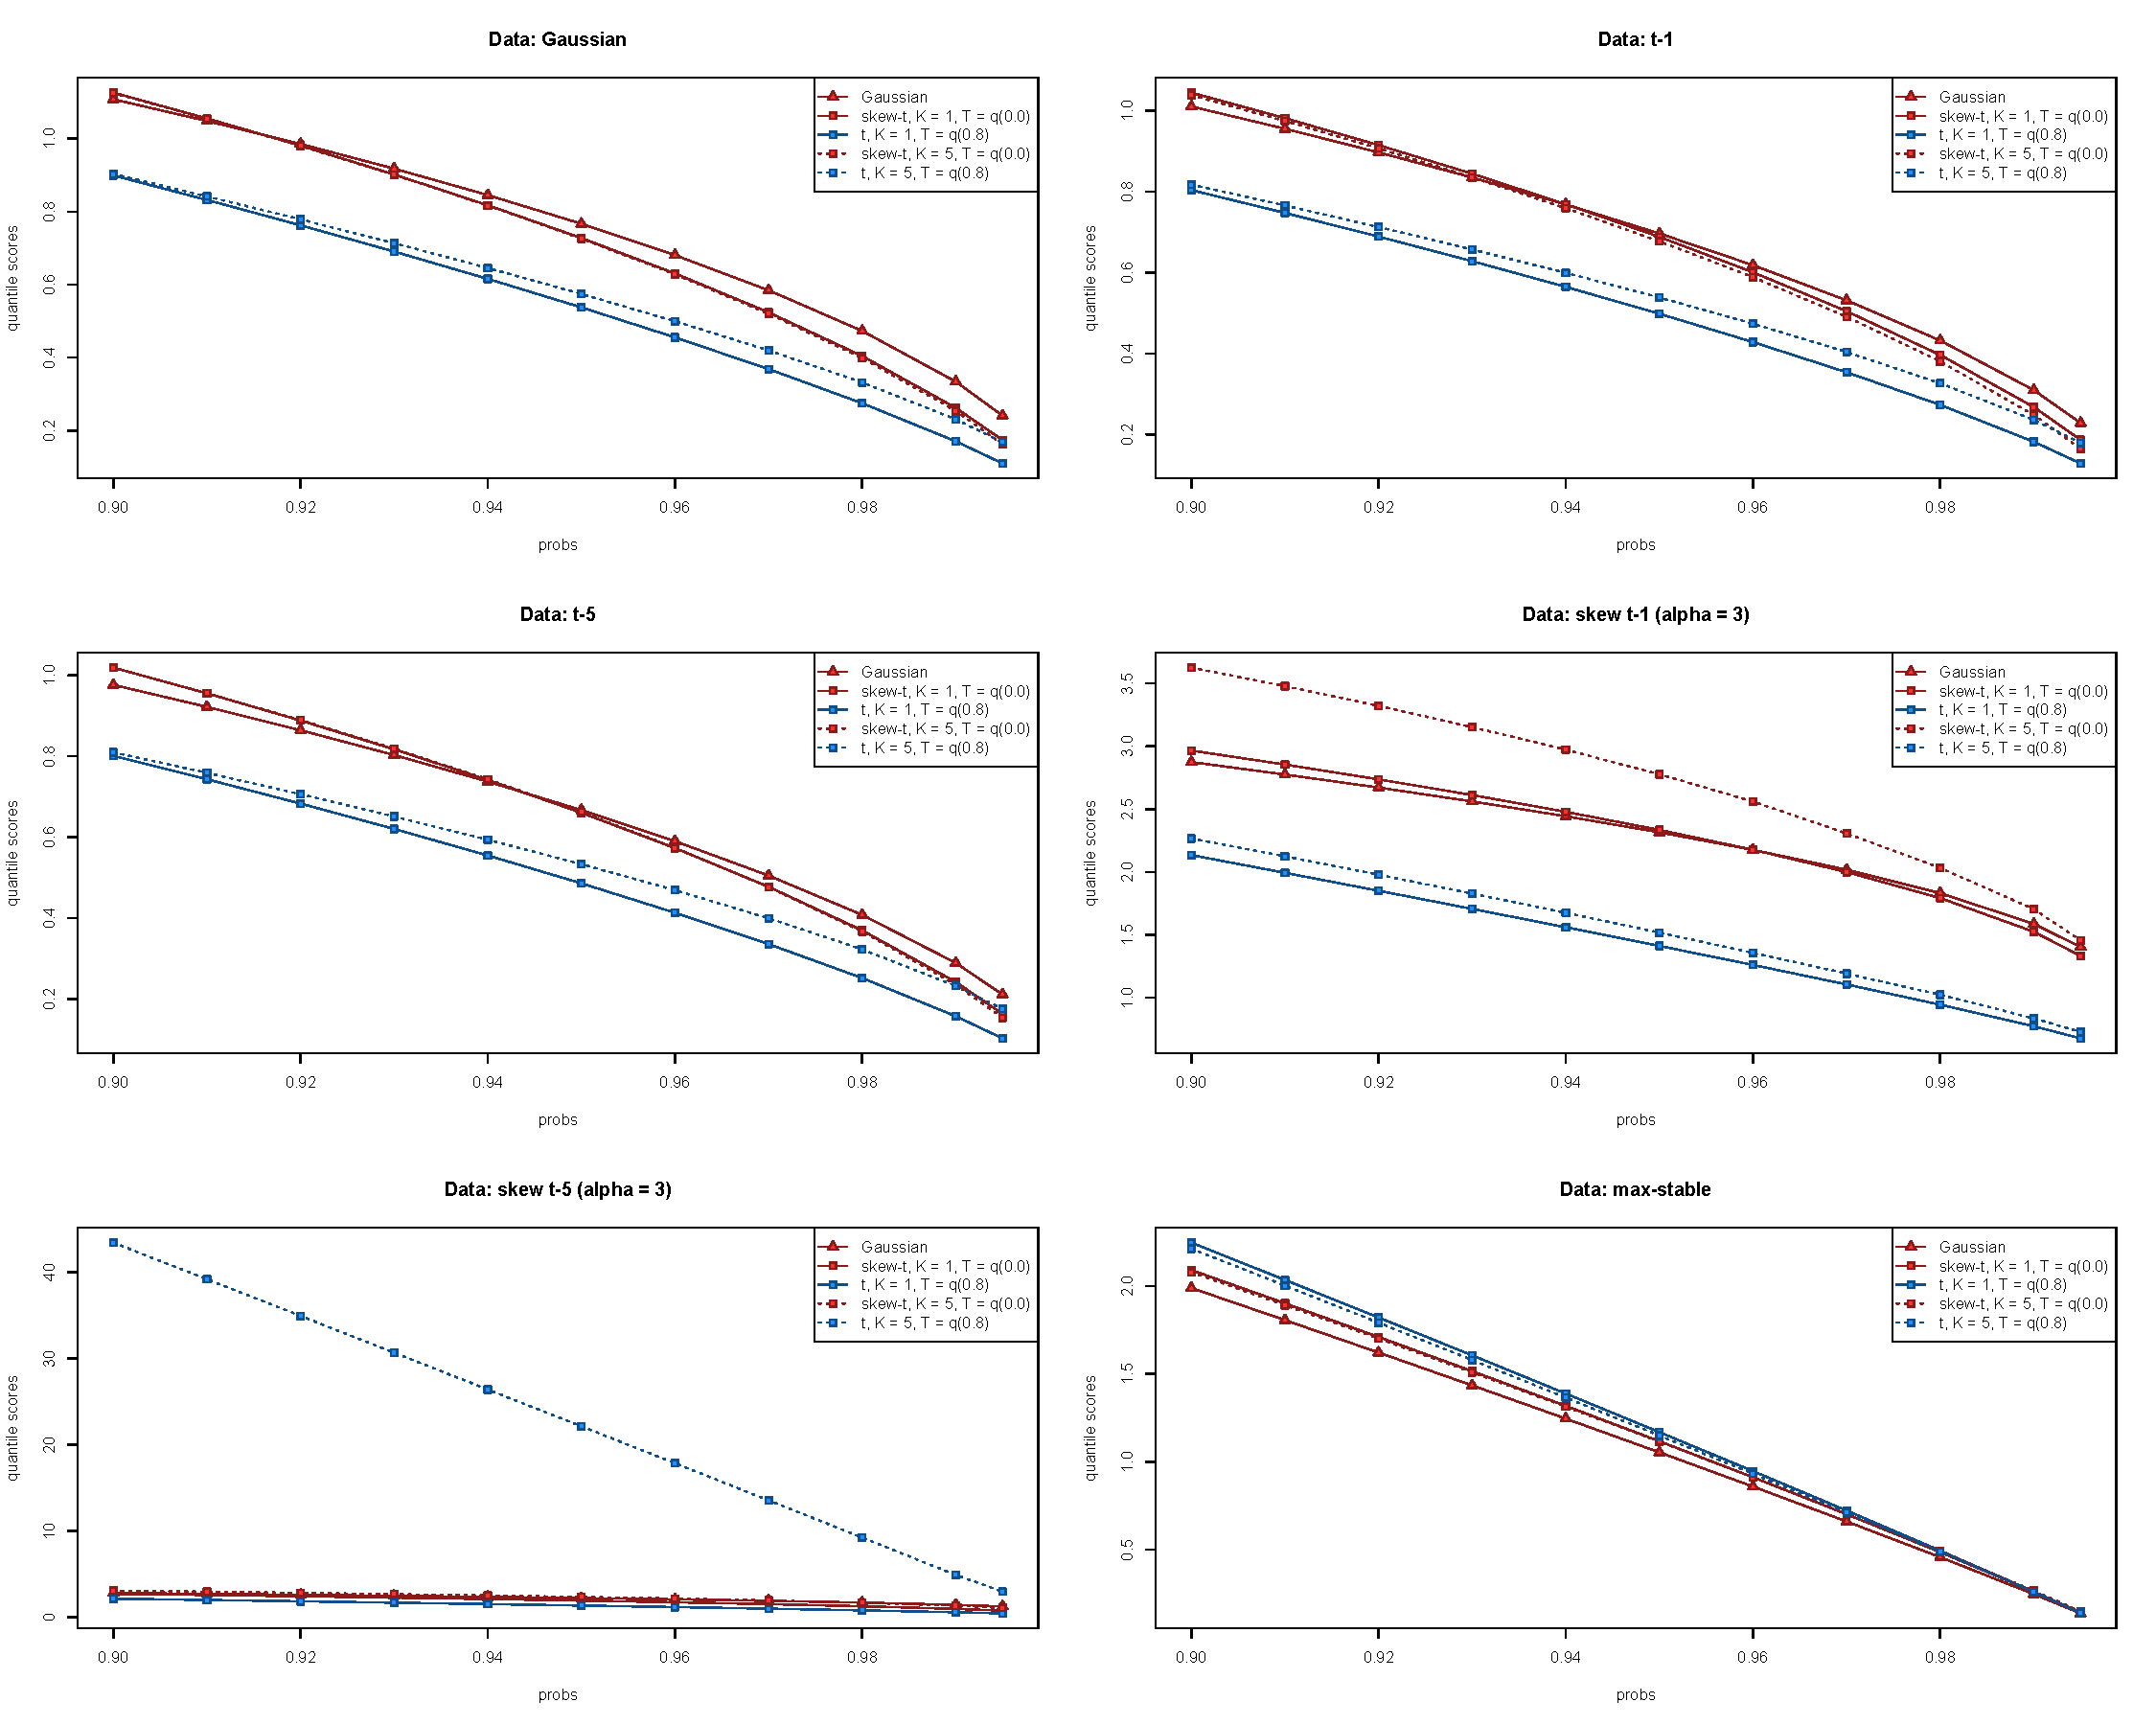
\includegraphics[width=\linewidth]{plots/quantileplots.pdf}
  \caption{Quantile score plots for simulation study results}
  \label{fig:simquantscores}
\end{figure}

\section{Data analysis}\label{s:analysis}
To illustrate this method, we consider the daily maximum 8-hour ozone measurements for July 2005 at 735 Air Quality System (AQS) monitoring sites in the eastern United States as the response.
For each site, we also have covariate information containing the estimated ozone from the Community Multi-scale Air Quality (CMAQ) modeling system.
Initially, we fit a linear regression assuming that the mean function can be expressed as
\begin{align}
  \mu_t(\bs) = \beta_0 + \beta_1 \cdot \text{CMAQ}_t(\bs). \label{eq:datamean}
\end{align}
The data from 10 July are shown in Figure \ref{fig:ozone} along with a Q-Q plot of the residuals compared to a skew-$t$ distribution with 8 d.f. and $\alpha = 1$.
\begin{center}
\begin{figure}
  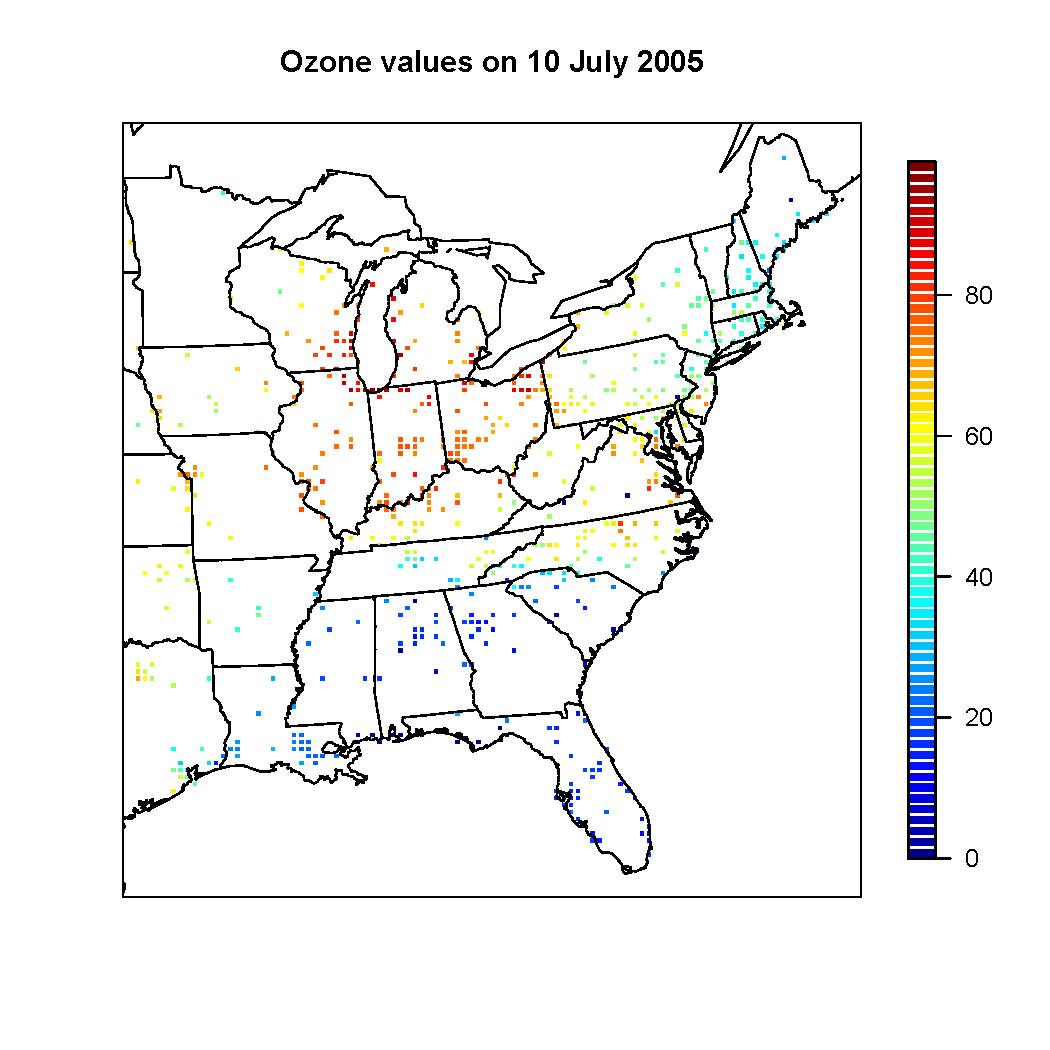
\includegraphics[width=0.5\linewidth]{plots/ozone-10jul.pdf}
  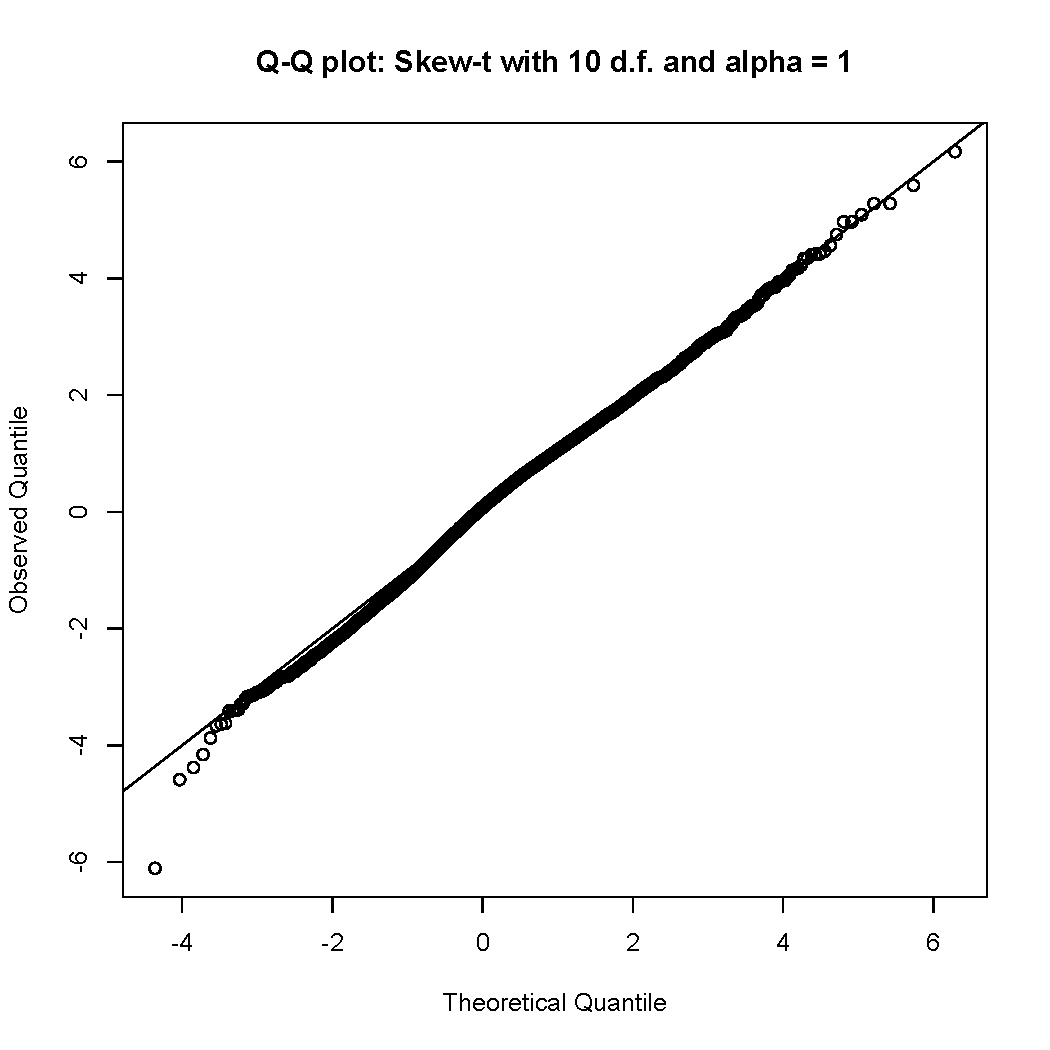
\includegraphics[width=0.5\linewidth]{plots/qq-res.pdf}
  \caption{Ozone values on 10 July 2005 (left) Q-Q plot of the residuals (right)}
  \label{fig:ozone}
\end{figure}
\end{center}
The $\chi(h)$ and $\chi(t)$ plots indicate that the residuals still demonstrate spatial and temporal dependence (see Figure \ref{fig:chi-st})
\begin{center}
\begin{figure}
  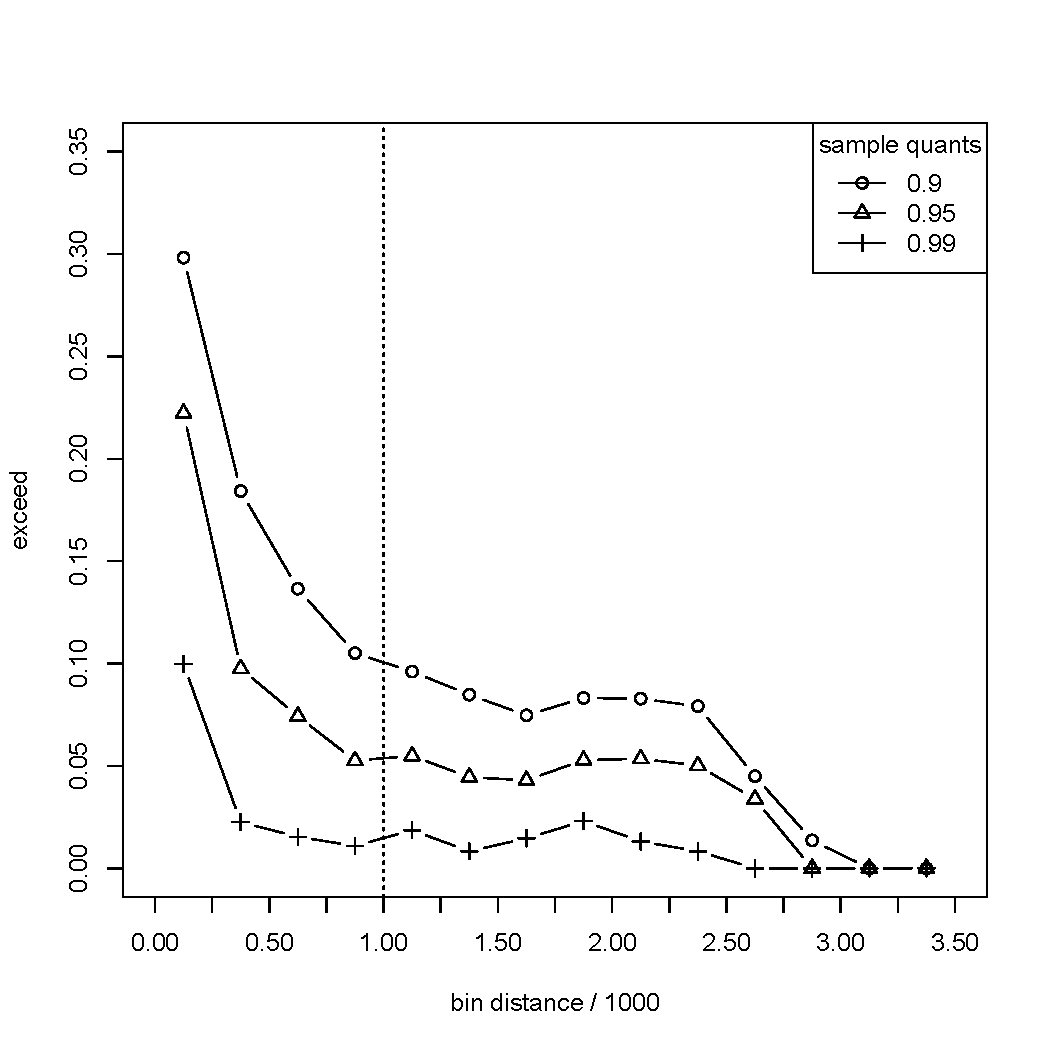
\includegraphics[width=0.5\linewidth]{plots/chi-h-ozone.pdf}
  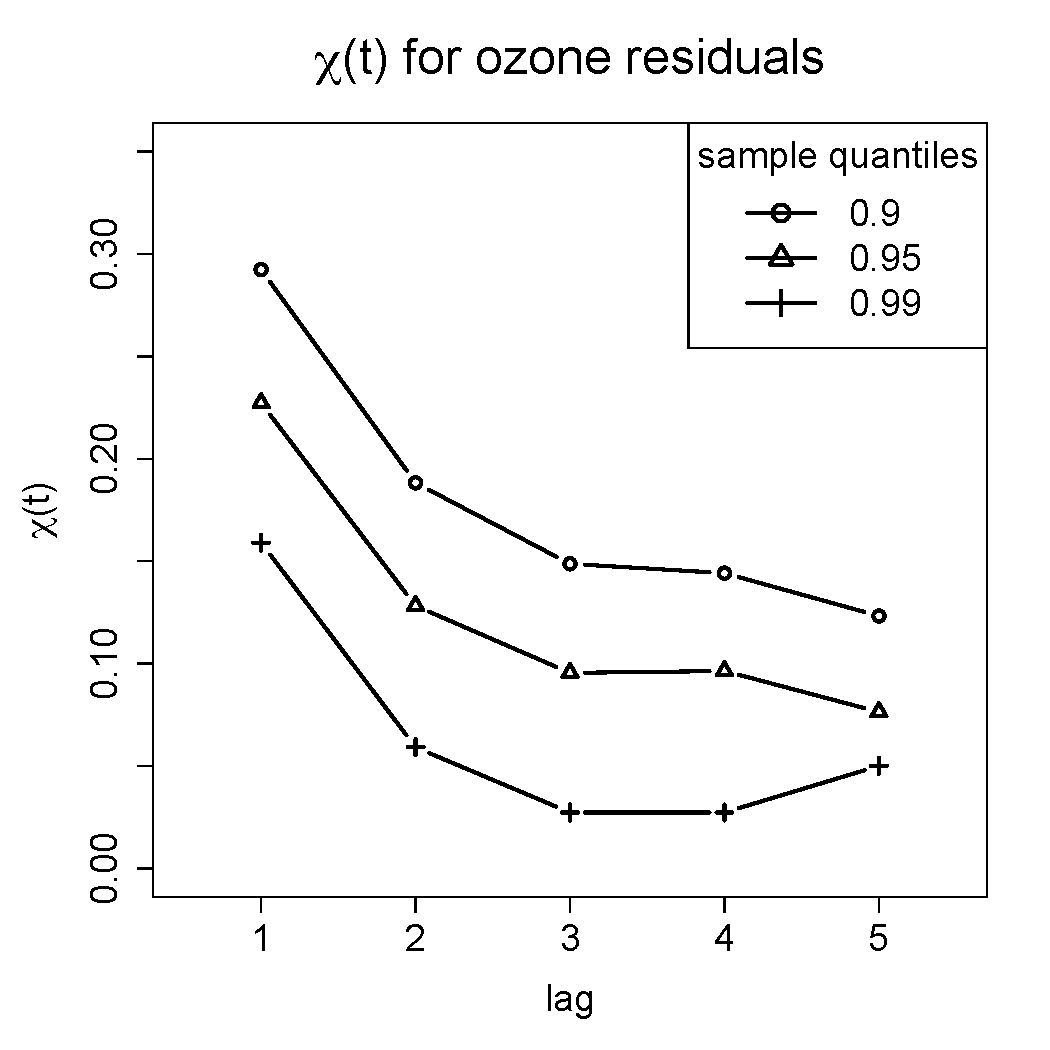
\includegraphics[width=0.5\linewidth]{plots/chi-t-ozone.pdf}
  \caption{$\chi(h)$ plot for the residuals. The vertical line indicates distance after which observations no longer demonstrate dependence (left) $\chi(t)$ plot for the residuals (right)}
  \label{fig:chi-st}
\end{figure}
\end{center}

\subsection{Model comparisons}
We fit the model using Gaussian and skew-$t$ marginal distributions, $K=1, 5, 10, 15$ partitions, with $Y(\bs)$ censored at $T = 0, 50, 75, 90$ ppb as described in Section \ref{s:data}.
We also include a max-stable analysis using the method by ????
All methods assume the mean function given in (\ref{eq:datamean}).
For each model, Brier scores and quantile scores were were averaged over all sites and days to obtain a single quantile score for each dataset.
At a particular threshold or quantile level, the model that fits the best is the one with the lowest score.
Looking at the heatplot in Figure \ref{fig:heatplot}, we can see that the methods using no thresholding tend to outperform those methods that do use thresholding.


\subsection{Results}\label{s:results}
\begin{figure}
  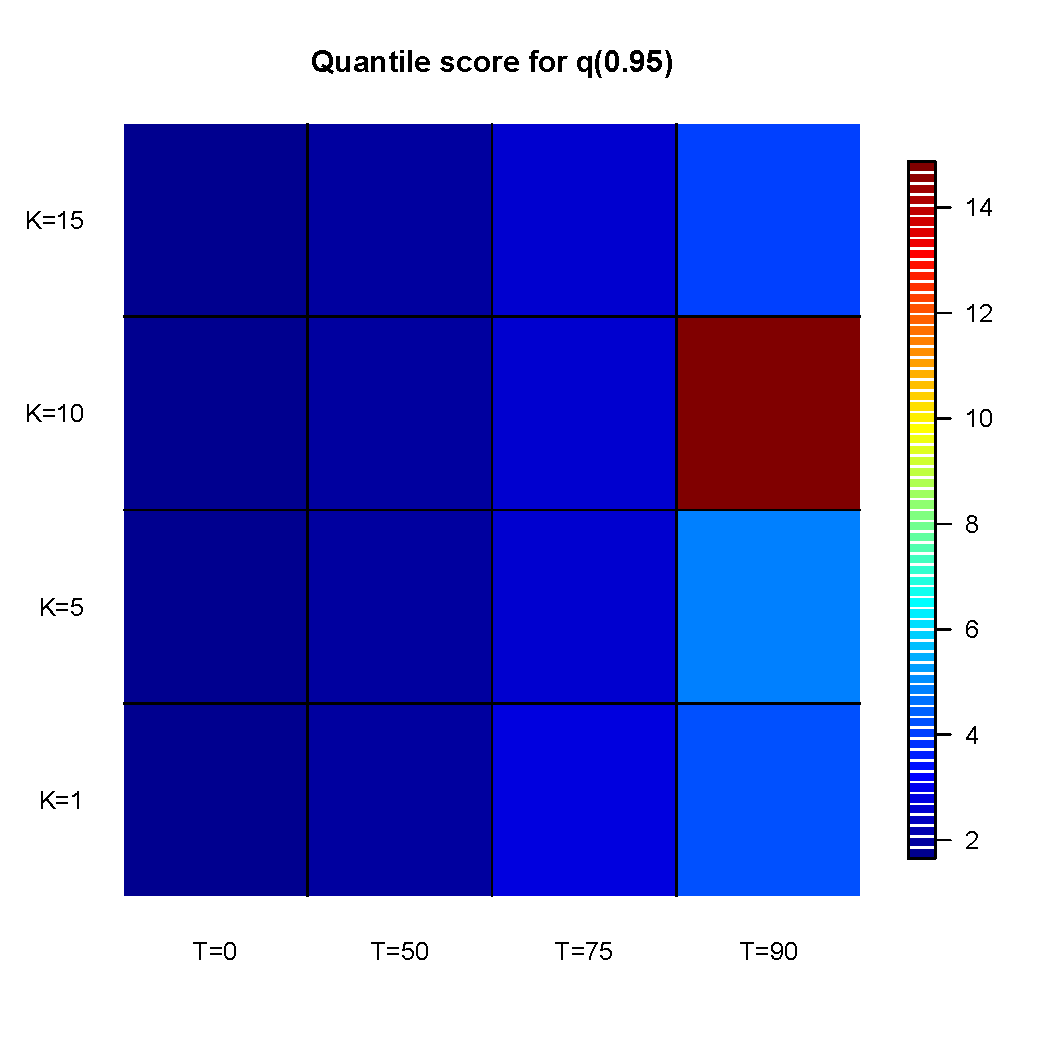
\includegraphics[width=0.5\linewidth]{plots/heatplot.pdf}
  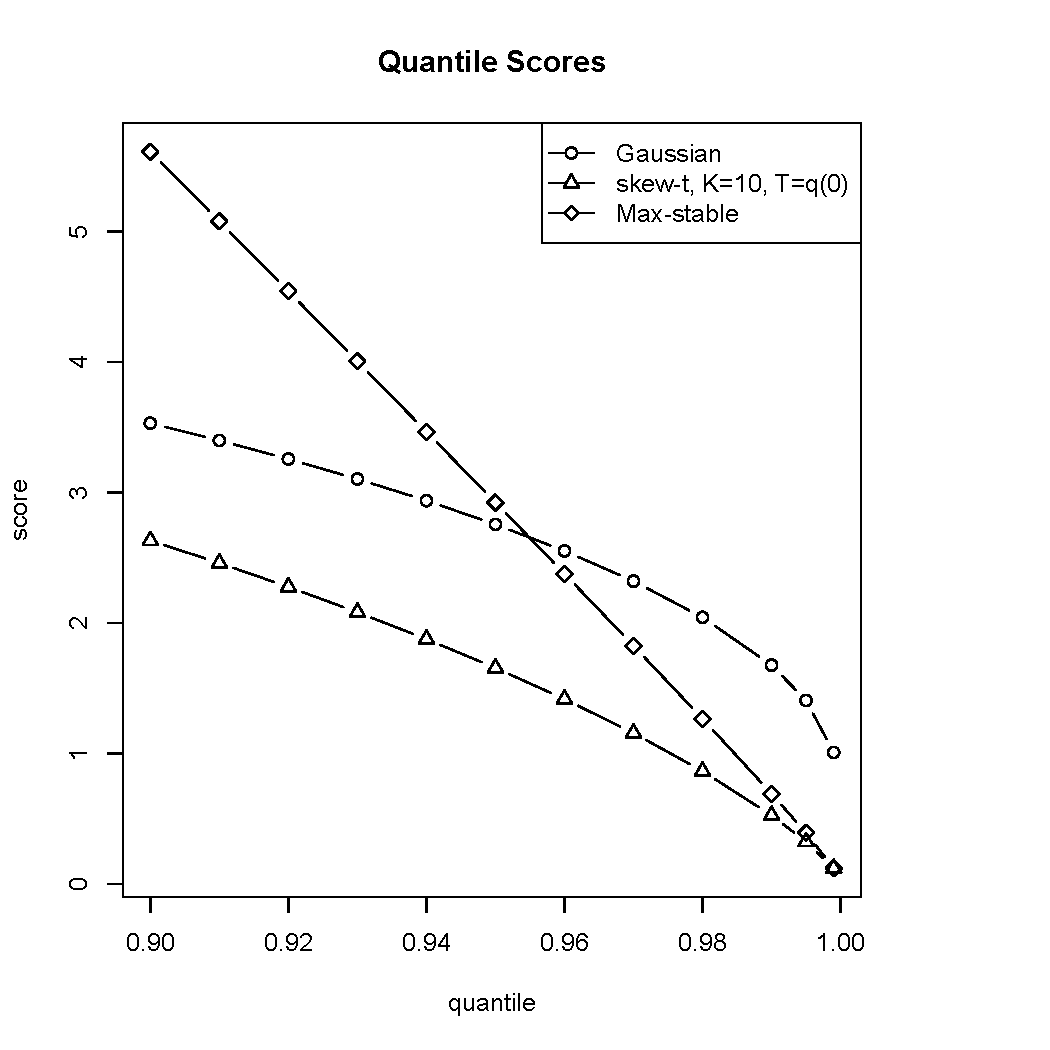
\includegraphics[width=0.5\linewidth]{plots/qscore-best.pdf}
  \caption{Heatplot of quantile scores for the 99th quantile (left) Quantile scores of Gaussian, skew-$t$ (K=10, T=q(0)), and Max-stable (right)}
  \label{fig:heatplot}
\end{figure}

\section{Conclusions}\label{s:con}

\section*{Acknowledgments}

\section*{Appendix A.1: MCMC details}
The MCMC sampling for the model \ref{s:hier} is done using {\tt R} (http://www.r-project.org). Whenever possible, we select conjugate priors (see Appendix A.2); however, for some of the parameters, no conjugate prior distributions exist.
When no conjugate prior distribution exists, we use a random walk Metropolis Hastings update step.
In each Metropolis Hastings update, we tune the algorithm to give acceptance rates near 0.40.

\subsection*{Spatial knot locations}
For each day, we update the spatial knot locations, $\bw_1, \ldots, \bw_K$, using a Metropolis Hastings block update.
Because the spatial domain is bounded, we generate candidate knots using the transformed knots $\bw^*_1, \ldots, \bw^*_K$ (see section \ref{s:hier}) and a random walk bivariate Gaussian candidate distribution
\begin{align*}
	{\bw^*_k}^{(c)} \sim \text{N}({\bw^*_k}^{(r - 1)}, s^2 I_2)
\end{align*}
where $\bw*_k^{(r - 1)}$ is the location for the transformed knot at MCMC iteration $r - 1$, $s$ is a tuning parameter, and $I_2$ is an identity matrix.
After candidates have been generated for all $K$ knots, the acceptance ratio is
\begin{align*}
  R = \left\{ \frac{ l[ Y_t(\bs | \bw_1^{(c)}, \ldots, \bw_K^{(c)}, \ldots)] }{l[ Y_t(\bs | \bw_1^{(r - 1)}, \ldots, \bw_K^{(r - 1)}, \ldots)]} \right\} \times \left\{ \frac{ \prod_{k = 1}^{K}\phi(\bw_k^{(c)})}{ \prod_{k = 1}^{K}\phi(\bw_k^{(r - 1)})} \right\}
\end{align*}
where $l$ is the likelihood given in (\ref{eq:hier}).
The candidate knots are accepted with probability $\min\{R, 1\}$.

\subsection*{Spatial random effects}
If there is temporal dependence amongst the observations, then we update $z_{tk}$, using a Metropolis Hastings update.
First, we generate a candidate using a random walk Gaussian candidate distribution
\begin{align*}
  z_{tk}^{(c)} \sim \text{N}(z_{tk}^{(r - 1)}, s^2)
\end{align*}
where $z_{tk}^{(r-1)}$ is the value at MCMC iteration $r - 1$, and $s$ is a tuning parameter.
The acceptance ratio is
\begin{align*}
  R = \left\{ \frac{ l[Y_t(\bs) | z_{tk}^{(c)}, \ldots] }{ l[Y_t(\bs) | z_{tk}^{(r - 1)}]} \right\} \times \left\{ \frac{ p[ z_{tk}^{(c)} ] }{ p[ z_{tk}^{(r - 1)}]}\right\}.
\end{align*}
The candidate is accepted with probability $\min\{R, 1\}$

\subsection*{Spatial covariance parameters}
We update the three spatial covariance parameters, $\log(\rho)$, $\log(\nu)$, $\gamma$, using a Metropolis Hastings block update step.
First, we generate a candidate using a random walk Gaussian candidate distribution
\begin{align*}
	\log(\rho)^{(c)} \sim \text{N}(\log(\rho)^{(r - 1)}, s^2)
\end{align*}
where $\log(\rho)^{(r-1)}$ is the value at MCMC iteration $r - 1$, and $s$ is a tuning parameter.
Candidates are generated for $\log(\nu)$ and $\gamma$ in a similar fashion.
The acceptance ratio is
\begin{align*}
	R = \left\{ \frac{ \prod_{t = 1}^{T} l[Y_t(\bs) | \rho^{(c)}, \nu^{(c)}, \gamma^{(c)}, \ldots] }{\prod_{t = 1}^{T} l[Y_t(\bs) | \rho^{(r-1)}, \nu^{(r-1)}, \gamma^{(r-1)}, \ldots] } \right\} \times \left\{ \frac{ p[\rho^{(c)}] }{ p[\rho^{(r - 1)] } } \right\} \times \left\{ \frac{ p[\nu^{(c)}] }{ p[\nu^{(r - 1)}] } \right\} \times \left\{ \frac{ p[ \gamma^{(c)} ] }{ p[\gamma^{(r - 1)} ] } \right\}.
\end{align*}
All three candidates are accepted with probability $\min\{R, 1\}$.

\section*{Appendix A.2: Posterior distributions}



%\subsubsection*{Conditional posterior of $U | Y$}\label{s:condu}
% Let $Y_i | U \sim \mbox{N}(U, \sigma^2)$, $i = 1, \ldots, n$, let $\tau = 1 / \sigma^2$, and let $\pi(U) \propto \exp \left\{ -\frac{ u^2 \theta }{ 2 } \right\}$. 
% Then the conditional posterior of $U \mid \ldots$ is 
% \begin{align}
%   \pi (U \mid \ldots) & \propto \exp \left\{ -\frac{ u^2 \theta }{ 2 } \right\} \exp \left\{ - \sum_{i = 1 }^n\frac{ \tau (y_i - u)^2 }{ 2 } \right\} \nonumber \\
%     & \propto \exp \left\{ -\frac{ 1 }{ 2 } \left[ u^2 \theta + \sum_{i=1 }^n\tau (y_i^2 - 2y_iu + u^2) \right] \right\} \nonumber \\
%     & \propto \exp \left\{ - \frac{ 1 }{ 2 }\left( u - \frac{ \tau \sum_{i=1}^n y_i }{ \theta + n \tau } \right)^2 \left( \theta + n \tau \right) \right\} \nonumber\\
%     & \propto \mbox{HN}(\xi^*, \theta^*) \label{eq:condu}
% \end{align}
% where 
% \begin{align*}
%   \xi^* &= \frac{ \tau \sum_{i=1}^n y_i }{ \theta + n \tau }\\
%   \theta^* &= \theta + n \tauå
% \end{align*}

\subsubsection*{Conditional posterior of $z_{tl} \mid \ldots $}\label{s:mvcondu}
For simplicity, drop the subscript $t$ and define 
\begin{align*}
R(\bs) = \left\{ 
    \begin{array}{ll}
        Y(\bs) - X(\bs) \beta &s \in P_l\\[1em]
        Y(\bs) - X(\bs) \beta - \delta z(\bs) \qquad & s \notin P_l
    \end{array} 
\right.
\end{align*}
Let 
\begin{align*}
    R_1 &= \text{the vector of } R(\bs) \text{ for } s \in P_l \\
    R_2 &= \text{the vector of } R(\bs) \text{ for } s \notin P_l \\
    \Omega &= \Sigma^{-1}.
\end{align*}
Then
\begin{align*}
    \pi(z_l | \ldots) &\propto \exp \left\{ -\frac{ 1 }{ 2 \sigma^2 } \left[ \frac{ 1 }{ (1 - \delta^2)}
        \left( \begin{array}{c}
            R_1 - \delta z_l \bOne\\
            R_2
        \end{array} \right)^T
        \left( \begin{array}{cc}
            \Omega_{11} & \Omega_{12}\\
            \Omega_{21} & \Omega_{22}
        \end{array} \right)
        \left( \begin{array}{c}
            R_1 - \delta z_l \bOne\\
            R_2
        \end{array} \right)
        +  z_l^2 \right]
    \right\} I(z_l > 0) \\
        &\propto \exp \left\{ -\frac{ 1 }{ 2 \sigma^2 } \left[ \Lambda_z z_l^2 - 2 \mu_z z_l \right] \right\} I(z_l > 0)
\end{align*}
where
\begin{align*}
    \mu_z &= \frac{ \delta}{(1 - \delta^2)} ( R_1^T \Omega_{11} + R_2^T \Omega_{21} )\bOne\\
    \Lambda_z &= \frac{\delta^2 \bOne^T \Omega_{11} \bOne }{ (1 - \delta^2) } + 1.
\end{align*}
Then $Z_l | \ldots \sim N_{(0, \infty)} (\Lambda_z^{-1} \mu_z, \sigma^2 \Lambda_z^{-1})$
\subsection*{Conditional posterior of $\beta \mid \ldots$}\label{s:betapost}
Let $\beta \sim \mbox{N}_{p}(0, \Lambda_0)$ where $\Lambda_0$ is a precision matrix. Then 
\begin{align*}
    \pi(\beta \mid \ldots) & \propto \exp \left\{ - \frac{ 1 }{ 2 } \beta^T \Lambda_0 \beta - \sum_{t = 1 }^T \frac{ 1 }{ 2 } [\bY_t(\bs) - X_t(\bs) \beta - \sigma \delta |u_t|]^T \Sigma^{-1} [\bY_t(\bs) - X_t(\bs) \beta - u^*_t] \right\}\\
     & \propto \exp \left\{ -\frac{ 1 }{ 2 } \left[ \beta^T \Lambda_p \beta  - \sum_{ t = 1 }^T 2 [ \beta^T X_t(\bs) \Sigma^{-1} (\bY_t(\bs) + u^*_t )] \right] \right\}\\
     & \propto \mbox{N}_p ( \mu_p , \Lambda_p)
\end{align*}
where
\begin{align*}
    \mu_p &= \Lambda_p^{-1} \left[ X_t(\bs)^T \Sigma^{-1} (\bY_t(\bs) + u^*_t) \right]\\
    \Lambda_p &= \left (\Lambda_0 + \sum_{ t = 1 }^{ T} X_t(\bs)^T \Sigma^{-1} X_t(\bs) \right)
\end{align*}
and $\Lambda_p$ is a precision matrix.
\subsection*{Conditional posterior of $\sigma^2 \mid \ldots$}\label{s:sigpost}
In the case where $L = 1$, then $\sigma^2$ has a conjugate posterior distribution. 
Let $\sigma_t^2 \iid \mbox{IG}(\alpha_0, \beta_0)$. For simplicity, drop the subscript $t$. Then
\begin{align*}
    \pi(\sigma^2 \mid \ldots) & \propto (\sigma^2)^{ -\alpha_0 - 1 / 2 - n / 2 - 1} \exp \left\{ -\frac{\beta_0}{\sigma^2} - \frac{ z^2 }{2 \sigma^2} - \frac{ (\bY - \bmu)^T \Sigma^{-1} (\bY - \bmu) }{2 \sigma^2} \right\} \\
    & \propto (\sigma^2)^{ -\alpha_0 - 1 / 2 - n / 2 - 1} \exp \left\{ - \frac{ 1 }{ \sigma^2 } \left[\beta_0 + \frac{ z^2 }{ 2 } + \frac{ 1 }{ 2 } (\bY - \bmu)^T \Sigma^{-1} (\bY - \mu) \right] \right\} \\
    & \propto \mbox{IG} (\alpha^*, \beta^*)
\end{align*}
where
\begin{align*}
    \alpha^* &= \alpha_0 + \frac{1}{2} + \frac{n}{2} \\
    \beta^* &= \beta_0 + \frac{ z^2 }{ 2 } + \frac{ 1 }{ 2 }(\bY - \bmu)^T \Sigma^{-1} (\bY - \bmu).
\end{align*}
In the case that $L > 1$, a random walk Metropolis Hastings step will be used to update $\sigma^2_{lt}$.
\subsection*{Conditional posterior of $\alpha \mid \ldots$}\label{s:alphapost}
Let $\alpha \sim N(0, \tau_\alpha)$ where $\tau_\alpha$ is a precision term. Then
\begin{align*}
  \pi(\alpha \mid \ldots) &\propto \exp \left\{ -\frac{ 1 }{ 2 } \tau_\alpha \alpha^2 + \sum_{ t = 1 }^T \frac{ 1 }{ 2 } [\bY_t - X_t\beta - \alpha |z_t|]^T \Omega [\bY_t - X_t\beta - \alpha |z_t|] \right\} \\
      &\propto \exp \left\{ -\frac{ 1 }{ 2 } [\alpha^2(\tau_\alpha + \sum_{t = 1 }^T |z_t|^T \Omega |z_t|^T) - 2 \alpha \sum_{t=1}^T[|z_t|^T \Omega (\bY_t - X_t \beta) \right\}\\
      &\propto \exp \left\{ -\frac{ 1 }{ 2 } [\tau_\alpha^* \alpha^2 - 2 \mu_\alpha] \right\}
\end{align*}
where
\begin{align*}
  \mu_\alpha &= \sum_{t = 1}^T |z_t|^T \Omega (\bY_t - X_t \beta)\\
  \tau_\alpha^* &= t_\alpha + \sum_{t=1}^T |z_t|^T \Omega |z_t|.
\end{align*}
Then $\alpha \mid \ldots \sim N(\tau^{*-1}_\alpha \mu_\alpha, \tau^{*-1}_\alpha) $

\section*{Appendix A.3: Proof that $\lim_{h \rightarrow \infty} \pi(h) = 0$}
Consider two points $\bs_1, \bs_2 \in \calD \subset \calR^2$. Let $\calD = B_{2h}(\bm)$ which is a ball of radius $h > 0$ centered at $\bm$, the midpoint between $\bs_1$ and $\bs_2$, and $h = ||\bs_1 - \bs_2||$. Let $w_1, \ldots, w_K \sim \text{Unif}(\calD)$ be a set of random knots uniformly distributed over $\calD$. Define $g(\bs_i) = \argmin_j || \bs_i - w_j ||$ to be the partition in which $\bs_i$ resides. Let $\pi(h) = \Pr[ g(\bs_1) = g(\bs_2)]$ be the probability that both sites are in the same partition. Then $\pi(h)$ is the probability that $w_j$ is the only knot in $(B_a(\bs_1) \cup B_b(\bs_2) \cap \calD)$ where $a = ||\bs_1 - w_j||$ and $b = ||\bs_2 - w_j||$.

\section*{Appendix A.4: Half-normal distribution}
Let $u = |z|$ where $Z \sim N(\mu, \sigma^2)$.
Specifically, we consider the case where $\mu = 0$. Then $U$ follows a half-normal distribution which we denote as $U \sim HN(0, 1)$, and the density is given by
\begin{align}
  f_U(u) = \frac{ \sqrt{2} }{ \sqrt{\pi \sigma^2} } \exp \left( - \frac{ u^2 }{ 2 \sigma^2 } \right) I(u > 0)
\end{align}
When $\mu = 0$, the half-normal distribution is also equivalent to a $N_{(0, \infty)}(0, \sigma^2)$ where $N_{(a, b)}(\mu, \sigma^2)$ represents a normal distribution with mean $\mu$ and standard deviation $\sigma$ that has been truncated below at $a$ and above at $b$.

\section*{Appendix A.5: Multivariate skew-$t$ distribution}
Let $Z_{0t} \sim \text{SN}_d(0, \bar{\Omega}, \alpha)$ be a $d$-dimensional skew-normal random variable.
Note, the relationship between $\bar{\Omega}$ and the \Matern covariance matrix given for (\ref{eq:fullmodel}) is given as follows
\begin{align*}
  \alpha &= \frac{ \delta }{ \sqrt{1 - \delta^2} } \\
  D_\delta &= (diag(1 - \delta))^{1/2}\\
  \bar{\Omega} &= D_\delta (\Sigma + \lambda \lambda^T) D_\delta \\
  \lambda &= D_\delta^{-1} \delta\\
\end{align*}
Let $\sigma_{tk}^2 \sim \chi^2_\nu / \nu$ where $\nu$ is the degrees of freedom.
Let $Z_{tk} = \sigma_{tk}^{-1} Z_{0, tk}$.
After marginalizing out the $\sigma_{tk}^2$ terms, $Z$ follows a multivariate skew-$t$ distribution, and the density is given by
\begin{align*}
  f_z(z) = 2 t_d(z; \bar{\Omega}, \nu) T \left( \alpha^T z \sqrt{ \frac{\nu + d}{\nu + Q(z)} }; \nu + d\right)
\end{align*}
where $Q(z) = z^T \bar{\Omega}^{-1}z$ and $T(\cdot; \rho)$ denotes the univariate Student's $t$ distribution function on $\rho$ degrees of freedom \citep{Azzalini2013}.

\bibliographystyle{rss}
\bibliography{skewnormal}

\end{document}

